\chapter{Review}

\section{Reinforcement learning by self-play}
The traditional algorithm involves training agent with help of expert data, guidance or hard coded heuristic in that domain. They also don't discover paths which was not present in data. Reinforcement learning through self-play \cite{alphagozero} is the state of art algorithm for board game agent. In this algorithm, the agent learns new things by themselves without any human intervention. This algorithm has three parts, self-play, training, selection of new best agent. The agent tries to improve on the previous version of itself. This type of algorithm was not possible before because it requires a lot of computating power. It is very different to other supervised algorithms which requires a good source of data and the model is dependent upon the noise in data. But in the above algorithm it does not require data from outside, rather it create data by selecting highly probable and rewarding moves.


\subsection{Self-play}
The agent learns from the examples created by its previous version. There is one neural network $f_{\theta}$ which predicts actions probability and probability of winning if it played with itself (meaning same policy) from that state. $$ (p,v) = f_{\theta}(s) $$. So $(p,v)$ is the prediction of the network. With the help of this network combined with tree search, it produces better strategy for agent in next iteration. The tree search involved is Monte Carlo Tree Search (MCTS) \cite{alphagozero}.


After doing serveral MCTS iterations, one can estimation action probability with the help of number of visits taken to other state after taking action $a$.
$ \pi_{a} $ $ \propto $ $N(s,a)^{\tau}$ where $N(s,a)$ is the number of time $a$ action has been taken from state $s$ and $\tau$ is temperature parameter. $z$ is win or lose at the end of game. So $(\pi,z)$ is the examples created after the self play and $\pi$ is supposed to be better policy than the $p$ because of the tree search simulations.
The exisiting method uses upper confidence bound for action selection. Our method differs here using different bound for action selection. The bound used are being KL-UCB \cite{klucb} and Thompson sampling \cite{thompson}
\subsection{Training}
As previously mentioned, there is one neural network with two head one predicting policy and other probability of wining. We train this neural network with $(\pi,z)$ data. 


$loss = (z-v)^{2} + \pi^{T}log(p)$ 
\subsection{Selection of Model}
Selection of neural network is done with the help of tournaments between the new trained version of neural network and the previous neural network which was before training with the new data. Depending upon the thresold we decide the new network as our best network or not.

\begin{figure}
    [!htb]\centering
    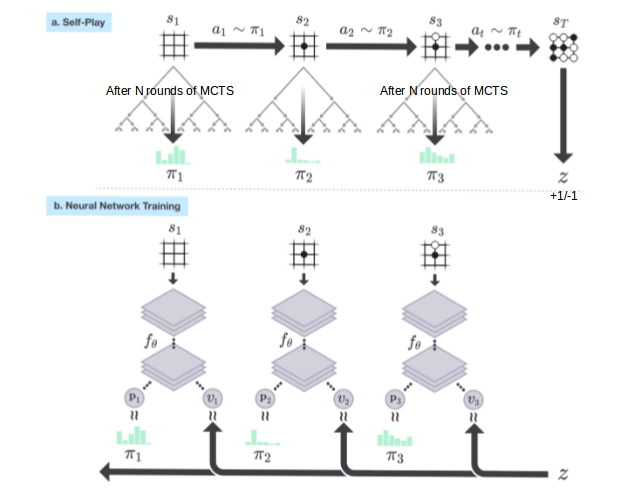
\includegraphics[width=6in]{images/selfplay.png}
    \caption{a. self-play: each action $a \sim \pi $ is done after N simulation and single example is created with values depending upon lose or win and probability depending upon number of actions taken. b. Neural network is trained with the examples created during self-play  }
  \label{fig:phase}
  \end{figure}

\section{Confidence bound}
So far Upper confidence bound is being using during the Monte Carlo Tree Search (MCTS)\cite{mcts} which minimize the regret.$$ A_{t} = argmax_{i}\; \left \lbrace Q_{i}(t-1) + c*P(s,a_{i}) \sqrt{\dfrac{2* \log N}{N_{i}}} \right \rbrace $$
$A_{t}$ is action taken at time $t$, $Q_{i}$ is average reward after taking $i^{th}$ action, $c$ is temperature parameter, $P(s,a_{i})$ is the probability of taking $i^{th}$ action in state $s$, $N$ is total number of simulations and $N_{i}$ is number of time $i^{th}$ action has been taken.



\section{Conclusion}
...................................



